% Shared by the paper and presentation. Dashed boxes are trust domains.
\resizebox{\linewidth}{!}{%
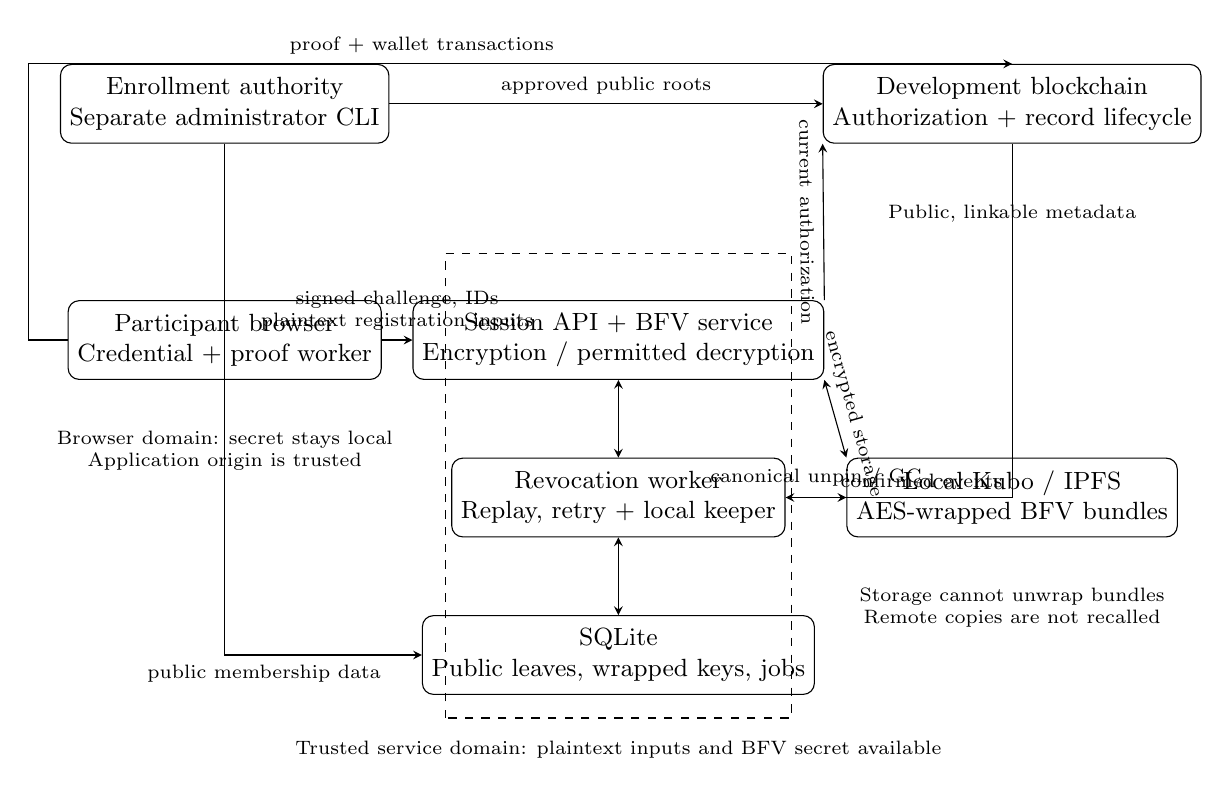
\begin{tikzpicture}[>=stealth,box/.style={draw,rounded corners,align=center,minimum width=3.3cm,minimum height=1cm,font=\small},every edge/.style={draw,->},every edge quotes/.style={font=\scriptsize}]
\node[box] (admin) at (-5,3) {Enrollment authority\\Separate administrator CLI};
\node[box] (browser) at (-5,0) {Participant browser\\Credential + proof worker};
\node[box] (chain) at (5,3) {Development blockchain\\Authorization + record lifecycle};
\node[box] (api) at (0,0) {Session API + BFV service\\Encryption / permitted decryption};
\node[box] (worker) at (0,-2) {Revocation worker\\Replay, retry + local keeper};
\node[box] (db) at (0,-4) {SQLite\\Public leaves, wrapped keys, jobs};
\node[box] (ipfs) at (5,-2) {Local Kubo / IPFS\\AES-wrapped BFV bundles};
\draw[dashed] (-2.2,-4.8) rectangle (2.2,1.1);
\node[font=\scriptsize,align=center] at (0,-5.2) {Trusted service domain: plaintext inputs and BFV secret available};
\draw[->] (admin) -- node[above,font=\scriptsize] {approved public roots} (chain);
\draw[->] (browser) -- node[above,font=\scriptsize,align=center] {signed challenge, IDs\\plaintext registration inputs} (api);
\draw[->] (browser.west) -- ++(-.5,0) |- node[pos=.7,above,font=\scriptsize] {proof + wallet transactions} (chain.north);
\draw[->] (api.north east) -- node[below,font=\scriptsize,sloped] {current authorization} (chain.south west);
\draw[->] (chain.south) |- node[pos=.7,above,font=\scriptsize] {confirmed events} (worker.east);
\draw[<->] (api) -- (worker);
\draw[<->] (worker) -- (db);
\draw[<->] (api.south east) -- node[above,font=\scriptsize,sloped] {encrypted storage} (ipfs.north west);
\draw[->] (worker) -- node[above,font=\scriptsize] {canonical unpin / GC} (ipfs);
\draw[->] (admin.south) |- node[pos=.6,below,font=\scriptsize] {public membership data} (db.west);
\node[font=\scriptsize,align=center] at (-5,-1.4) {Browser domain: secret stays local\\Application origin is trusted};
\node[font=\scriptsize,align=center] at (5,1.6) {Public, linkable metadata};
\node[font=\scriptsize,align=center] at (5,-3.4) {Storage cannot unwrap bundles\\Remote copies are not recalled};
\end{tikzpicture}%
}
